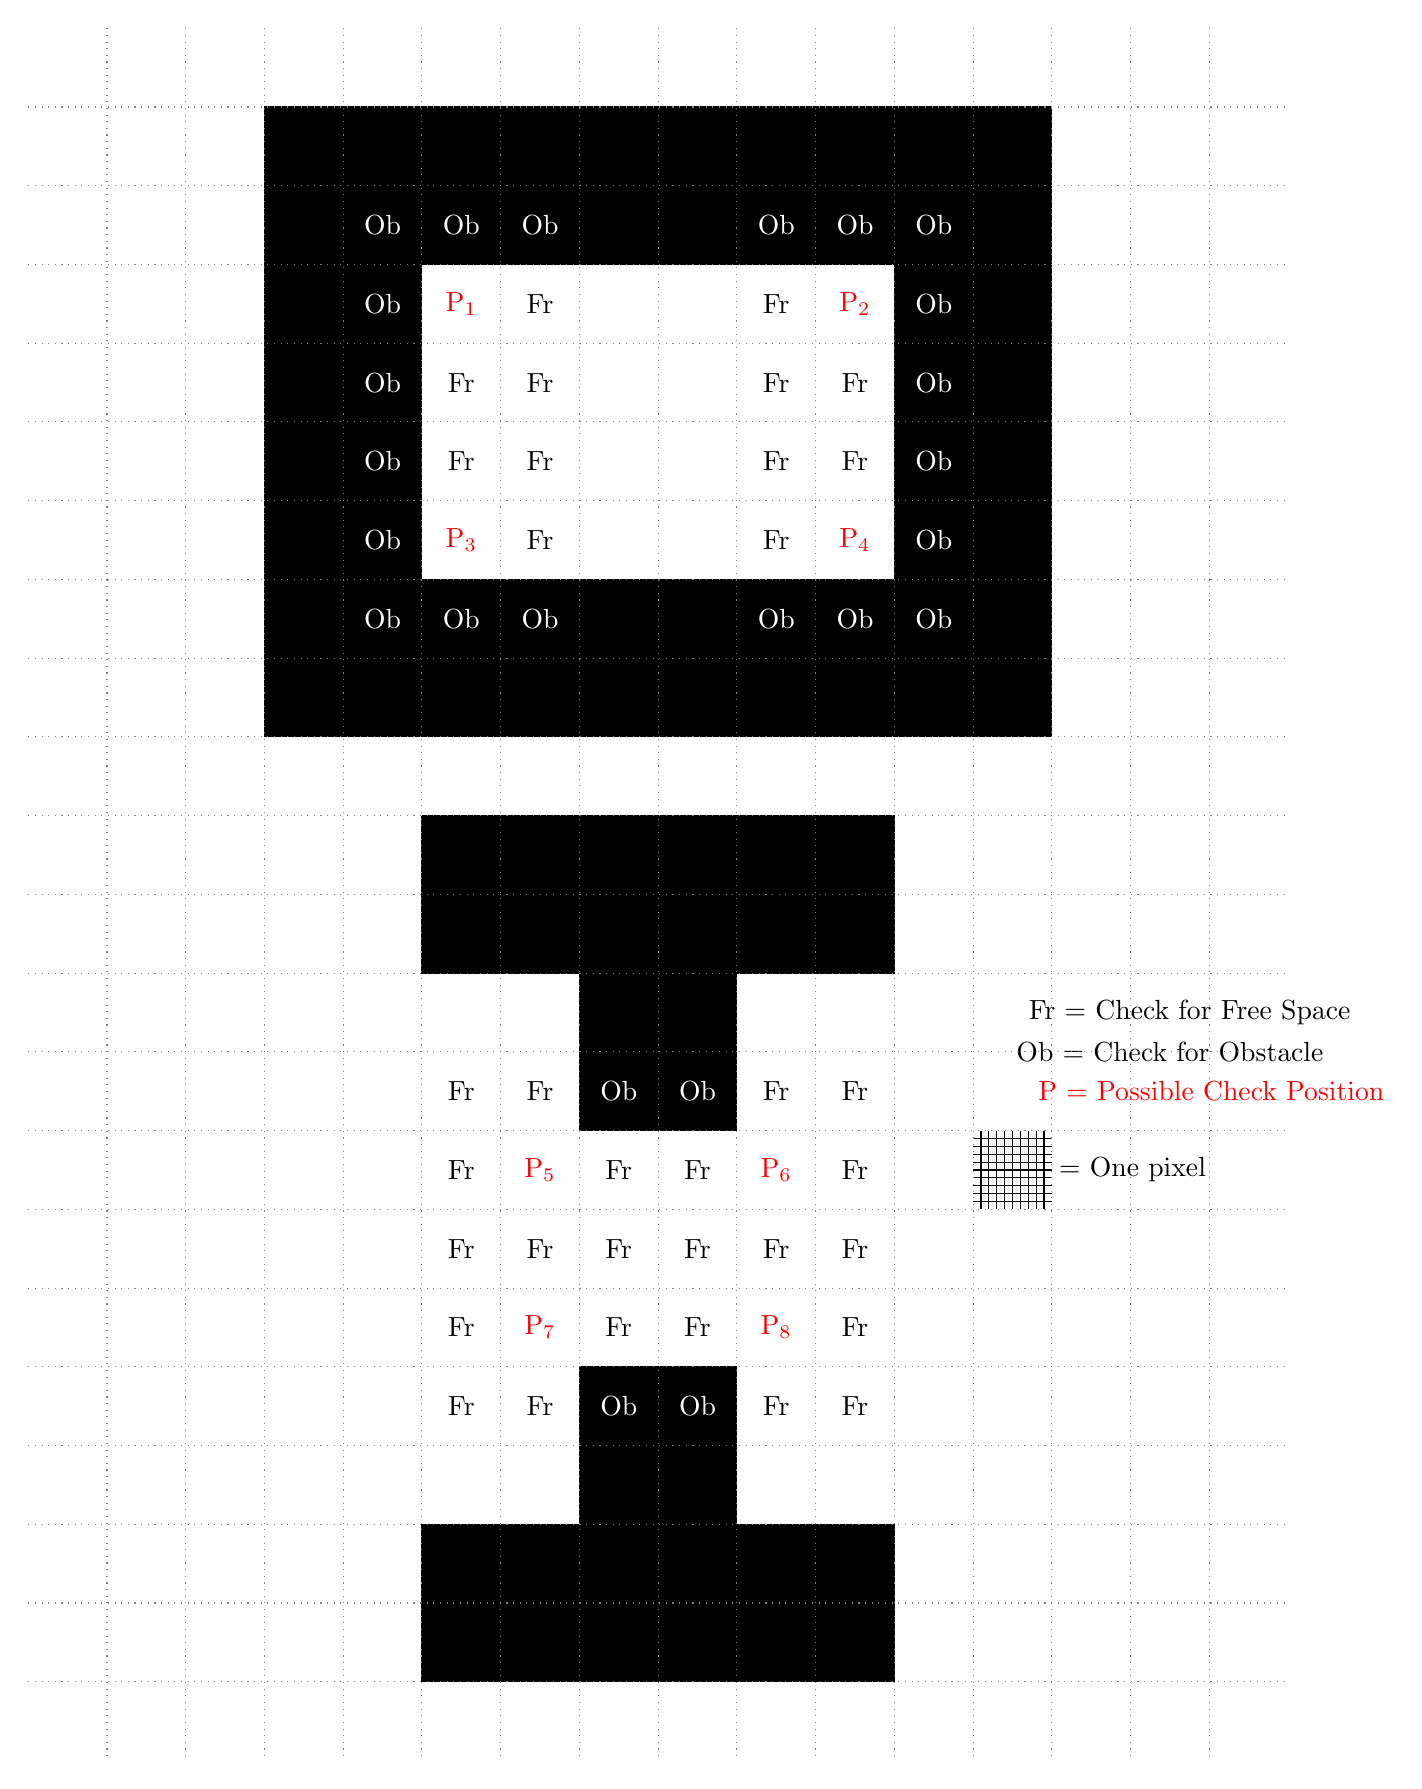
\begin{tikzpicture}[scale=1]


% Obstacles
\draw[fill=black](-3,-8)--++(2,0)--++(0,2)--++(2,0)--++(0,-2)--++(2,0)--++(0,-2)--++(-6,0)--++(0,2);
\draw[fill=black](-3,1)--++(6,0)--++(0,-2)--++(-2,0)--++(0,-2)--++(-2,0)--++(0,2)--++(-2,0)--++(0,2);
\draw[fill=black](-5,10)--++(10,0)--++(0,-8)--++(-10,0)--++(0,8);
\draw[fill=white](-3,8)--++(6,0)--++(0,-4)--++(-6,0)--++(0,4);

% Possible positions:
\node[color=red] at (2.5,4.5) {P\(_{4}\)};
\node[color=red] at (-2.5,4.5) {P\(_{3}\)};
\node[color=red] at (2.5,7.5) {P\(_{2}\)};
\node[color=red] at (-2.5,7.5) {P\(_{1}\)};

\node[color=red] at (1.5,-3.5) {P\(_{6}\)};;
\node[color=red] at (-1.5,-3.5) {P\(_{5}\)};;
\node[color=red] at (1.5,-5.5) {P\(_{8}\)};
\node[color=red] at (-1.5,-5.5) {P\(_{7}\)};;

% Check for obstacles 
\node[color=white] at (-3.5,5.5) {Ob};
\node[color=white] at (-3.5,4.5) {Ob};
\node[color=white] at (-3.5,3.5) {Ob};
\node[color=white] at (-2.5,3.5) {Ob};
\node[color=white] at (-1.5,3.5) {Ob};

\node[color=white] at (3.5,5.5) {Ob};
\node[color=white] at (3.5,4.5) {Ob};
\node[color=white] at (3.5,3.5) {Ob};
\node[color=white] at (2.5,3.5) {Ob};
\node[color=white] at (1.5,3.5) {Ob};

\node[color=white] at (3.5,6.5) {Ob};
\node[color=white] at (3.5,7.5) {Ob};
\node[color=white] at (3.5,8.5) {Ob};
\node[color=white] at (2.5,8.5) {Ob};
\node[color=white] at (1.5,8.5) {Ob};

\node[color=white] at (-3.5,6.5) {Ob};
\node[color=white] at (-3.5,7.5) {Ob};
\node[color=white] at (-3.5,8.5) {Ob};
\node[color=white] at (-2.5,8.5) {Ob};
\node[color=white] at (-1.5,8.5) {Ob};

\node[color= white] at (-0.5,-2.5) {Ob};
\node[color=white] at (0.5,-2.5) {Ob};

\node[color= white] at (-0.5,-6.5) {Ob};
\node[color=white] at (0.5,-6.5) {Ob};

% Check for free space
\node at (0.5,-3.5) {Fr};
\node at (-0.5,-3.5) {Fr};

\node at (0.5,-4.5) {Fr};
\node at (-0.5,-4.5) {Fr};

\node at (0.5,-5.5) {Fr};
\node at (-0.5,-5.5) {Fr};

\node at (1.5,-4.5) {Fr};
\node at (-1.5,-4.5) {Fr};

\node at (1.5,-6.5) {Fr};
\node at (-1.5,-6.5) {Fr};

\node at (1.5,-2.5) {Fr};
\node at (-1.5,-2.5) {Fr};

\node at (2.5,-2.5) {Fr};
\node at (-2.5,-2.5) {Fr};
\node at (2.5,-3.5) {Fr};
\node at (-2.5,-3.5) {Fr};
\node at (2.5,-4.5) {Fr};
\node at (-2.5,-4.5) {Fr};
\node at (2.5,-5.5) {Fr};
\node at (-2.5,-5.5) {Fr};
\node at (2.5,-6.5) {Fr};
\node at (-2.5,-6.5) {Fr};


\node at (2.5,6.5) {Fr};
\node at (-2.5,6.5) {Fr};
\node at (2.5,5.5) {Fr};
\node at (-2.5,5.5) {Fr};

\node at (1.5,4.5) {Fr};
\node at (-1.5,4.5) {Fr};

\node at (1.5,5.5) {Fr};
\node at (-1.5,5.5) {Fr};

\node at (1.5,6.5) {Fr};
\node at (-1.5,6.5) {Fr};
\node at (1.5,7.5) {Fr};
\node at (-1.5,7.5) {Fr};

% Description
\node[color=red] at (7.025,-2.5) {P = Possible Check Position};
\node at (6.5,-2) {Ob = Check for Obstacle};
\node at (6.75,-1.5) {Fr = Check for Free Space};
\node at (6.025,-3.5) {= One pixel};

\draw(4,-3.1)--++(1,0);
\draw(4,-3.2)--++(1,0);
\draw(4,-3.3)--++(1,0);
\draw(4,-3.4)--++(1,0);
\draw(4,-3.5)--++(1,0);
\draw(4,-3.6)--++(1,0);
\draw(4,-3.7)--++(1,0);
\draw(4,-3.8)--++(1,0);
\draw(4,-3.9)--++(1,0);

\draw(4.1,-3)--++(0,-1);
\draw(4.2,-3)--++(0,-1);
\draw(4.3,-3)--++(0,-1);
\draw(4.4,-3)--++(0,-1);
\draw(4.5,-3)--++(0,-1);
\draw(4.6,-3)--++(0,-1);
\draw(4.7,-3)--++(0,-1);
\draw(4.8,-3)--++(0,-1);
\draw(4.9,-3)--++(0,-1);



% V lines
\draw[dotted,color=gray](-7,11)--++(0,-22);
\draw[dotted,color=gray](-6,11)--++(0,-22);
\draw[dotted,color=gray](-5,11)--++(0,-22);
\draw[dotted,color=gray](-4,11)--++(0,-22);
\draw[dotted,color=gray](-3,11)--++(0,-22);
\draw[dotted,color=gray](-2,11)--++(0,-22);
\draw[dotted,color=gray](-1,11)--++(0,-22);
\draw[dotted,color=gray](0,11)--++(0,-22);
\draw[dotted,color=gray](7,11)--++(0,-22);
\draw[dotted,color=gray](6,11)--++(0,-22);
\draw[dotted,color=gray](5,11)--++(0,-22);
\draw[dotted,color=gray](4,11)--++(0,-22);
\draw[dotted,color=gray](3,11)--++(0,-22);
\draw[dotted,color=gray](2,11)--++(0,-22);
\draw[dotted,color=gray](1,11)--++(0,-22);

% H lines
\draw[dotted,color=gray](-8,10)--++(16,0);
\draw[dotted,color=gray](-8,9)--++(16,0);
\draw[dotted,color=gray](-8,8)--++(16,0);
\draw[dotted,color=gray](-8,7)--++(16,0);
\draw[dotted,color=gray](-8,6)--++(16,0);
\draw[dotted,color=gray](-8,5)--++(16,0);
\draw[dotted,color=gray](-8,4)--++(16,0);
\draw[dotted,color=gray](-8,3)--++(16,0);
\draw[dotted,color=gray](-8,2)--++(16,0);
\draw[dotted,color=gray](-8,1)--++(16,0);
\draw[dotted,color=gray](-8,0)--++(16,0);
\draw[dotted,color=gray](-8,-10)--++(16,0);
\draw[dotted,color=gray](-8,-9)--++(16,0);
\draw[dotted,color=gray](-8,-8)--++(16,0);
\draw[dotted,color=gray](-8,-7)--++(16,0);
\draw[dotted,color=gray](-8,-6)--++(16,0);
\draw[dotted,color=gray](-8,-5)--++(16,0);
\draw[dotted,color=gray](-8,-4)--++(16,0);
\draw[dotted,color=gray](-8,-3)--++(16,0);
\draw[dotted,color=gray](-8,-2)--++(16,0);
\draw[dotted,color=gray](-8,-1)--++(16,0);




\end{tikzpicture}